\documentclass[11pt]{book}
\usepackage{hyperref}
\usepackage{amsfonts}
\usepackage{amssymb}
\usepackage{amsmath}
\usepackage[utf8]{inputenc}
\usepackage[T1]{fontenc}
\usepackage{float}
\usepackage{fixltx2e}
\usepackage[italian]{babel}
\usepackage{graphicx}

\newenvironment{sistema}%
{\left\lbrace\begin{array}{@{}l@{}}}%
{\end{array}\right.}


\title{Appunti di Ricerca Operativa}
\author{Fabio Viola}
\date{}

\setcounter{chapter}{4}

\begin{document}

\chapter{Dualit\`a}

\scriptsize
{\bf Slide}:
\href{http://www.or.deis.unibo.it/staff_pages/martello/Chapter5.zip}{Duality}
\normalsize
\vspace{20pt}

\section{Duale di un problema in forma standard}

Consideriamo un problema LP in forma standard:

\vspace{11pt}
\begin{center}
\begin{tabular}{l}
$min\phantom{a}c'x$ \\
$\phantom{mina}Ax= b$ \\
$\phantom{mina}x\geq 0$ \\
\end{tabular}
\end{center}
\vspace{11pt}

Possiamo indicare con $Y$ la matrice $m \times n$ contenuta nelle
righe $1, \dots, m$ e nelle colonne $1, \dots, n$ del tableau. La
matrice {\em Y} \`e prodotta ad ogni iterazione dal prodotto

\begin{center}
$Y = B^{-1}A$  
\end{center}

dove $B^{-1}$ \`e l'inversa della matrice $B$ associata alla base
$\mathcal{B} = \{A_{\beta(1)},\dots,A_{\beta(m)} \}$. La matrice {\em
  Y} conterr\`a sempre un'identit\`a come base, mentre la base
$\mathcal{B}$ potrebbe in generale non avere una matrice identit\`a
come matrice associata.

A questo punto per\`o \`e necessario calcolare la riga 0, che come
abbiamo visto non fa parte di {\em Y}. I costi da inserire in riga 0
sono calcolati come:

\begin{center}
$\bar{c}' = c' - z'$ 
\end{center}

(e per il criterio di ottimalit\`a dobbiamo avere $\bar{c}'\geq 0$).

Esplicitiamo la precedente formula:

\begin{itemize}
\item $c'$: i termini di questo vettore corrispondono ai coefficienti
  delle variabili nell'equazione del problema;

\item $z' = c_\beta' Y = c_\beta' B^{-1}A$: il vettore $c_\beta'$
  contiene i coefficienti associati alle variabili in base.
\end{itemize}

Concentriamoci proprio su quest'equazione,
$c'-(c_\beta'B^{-1})A$. Sapendo che $c'$ e $A$ sono dati di input,
e pertanto noti, l'unica parte incognita \`e
$c_\beta'B^{-1}$. Possiamo indicare tale parte con $\pi'$, un vettore
di {\em m} elementi. Sostituendo abbiamo:

\begin{center}
$c'-\pi'A \geq 0$
\end{center}

dunque

\begin{center}
$\pi'A \leq c'$
\end{center}

$\pi'$ \`e prodotto dalla base ottima se \`e soluzione ammissibile del
sistema di {\em n} disequazioni lineari in {\em m} incognite appena
trovato. \`E emerso perci\`o un nuovo problema di programmazione
lineare in cui, lo vediamo osservando bene, i vincoli sono dati dalle
colonne di {\em A} e i termini noti sono i costi. Provando a
formalizzare tale problema possiamo definire il {\bf problema duale}:

\vspace{11pt}
\begin{center}
\begin{tabular}{l}
$\max \pi'b$ \\
$\phantom{mina}\pi'A \leq c'$ \\
$\phantom{mina}\pi \gtreqless 0$ \\
\end{tabular}
\end{center}
\vspace{11pt}

Vedremo pi\`u avanti che $\mathcal{B}$ \`e base ottima dell'LP se e
solo se $\pi'$ \`e soluzione ottima del duale.

\vspace{11pt}
$\blacktriangleright$ {\bf Esempio}: consideriamo il seguente
problema:

\vspace{11pt}
\begin{center}
\begin{tabular}{l}
$\min z = 2x_1 + 3x_2 + x_3$\\
$\phantom{min z}2x_1 + x_2 = 1$\\
$\phantom{min z}x_1 + x_3 = 4$\\
$\phantom{min z}x_1,x_2,x_3 \geq 0$\\
\end{tabular}
\end{center}
\vspace{11pt}

Il problema, il cui tableau corrispondente \`e a sinistra in figura
\ref{cap5tab1}, e incidentalmente contiene gi\`a una base.

\begin{figure}[h!]
  \centering
  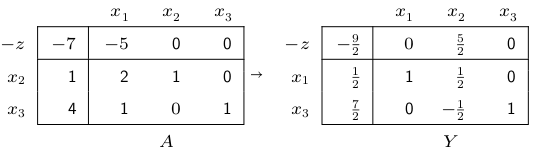
\includegraphics[width=0.7\textwidth]{images/cap5tab1.png}
  \caption{Figura d'esempio}
  \label{cap5tab1}
\end{figure}

La soluzione non \`e ancora quella ottima in quanto nella riga dei
costi vediamo che una colonna ha costo negativo. \`E necessario dunque
effettuare un pivoting e lo si fa sull'elemento cerchiato (che abbiamo
individuato tramite le regole note dai precedenti
capitoli). L'operazione che ci consente di effettuare il pivoting ed
ottenere il nuovo tableau pu\`o essere scritta come:

\begin{center}
$B^{-1}A = Y$  
\end{center}

dove {\em A} \`e la matrice dei coefficienti dei vincoli, {\em B} \`e
la matrice corrispondente alla base $\mathcal{B} = \{ A_2, A_3\}$ ed
{\em Y} \`e il nuovo tableau risultante esclusa la riga 0. Vediamo nel
dettaglio i calcoli:

\vspace{11pt}
\begin{center}
\begin{tabular}{lll}
$B = 
\begin{bmatrix}
  2 & 0 \\
  1 & 1 \\
\end{bmatrix}
$ &
$B^{-1} = 
\begin{bmatrix}
  \frac{1}{2} & 0 \\
  -\frac{1}{2} & 1 \\
\end{bmatrix}
$ &
$A =
\begin{bmatrix}
1 & 2 & 1 & 0 \\
4 & 1 & 0 & 1 \\
\end{bmatrix}
$ \\
&
\end{tabular}
\vspace{11pt}

\begin{tabular}{l}
$Y = 
\begin{bmatrix}
  \frac{1}{2} & 1 & \frac{1}{2} & 0 \\
  \frac{7}{2} & 0 & -\frac{1}{2} & 1 \\
\end{bmatrix}$
\end{tabular}
\end{center}
\vspace{11pt}

Ottenuto {\em Y} bisogna per\`o calcolare i costi e per far ci\`o
sfrutteremo i vettori $c' = \begin{bmatrix}2 & 3 & 1\end{bmatrix}$
  (che corrispondono ai coefficienti del problema) e $c_\beta'
  = \begin{bmatrix}2 &1 \end{bmatrix}$ che corrisponde al vettore dei
  coefficienti delle variabili in base (variabili che sono $x_1$ e
  $x_3$):

\vspace{11pt}
\begin{center}
\begin{tabular}{l}
$c_\beta'Y = z' = \begin{bmatrix}2 & 1\end{bmatrix}Y
    = \begin{bmatrix}2 & \frac{1}{2}& 1\end{bmatrix}$ \\
$c' - z' = \begin{bmatrix}2 & 3 & 1\end{bmatrix} - \begin{bmatrix}2 &
          \frac{1}{2} & 1\end{bmatrix} = \begin{bmatrix}0 &
            \frac{5}{2} & 0\end{bmatrix}$
\end{tabular}
\end{center}
\vspace{11pt}

e possiamo dunque completare il tabelau come vediamo in figura
\ref{cap5tab1} a destra. Vediamo ora come costruire il problema duale.

Avremo un problema di massimo e come variabili avremo $\pi'$ con
coefficienti i vecchi termini noti {\em b} e dato che gli elementi
$\pi'$ sono legati alla base ed essendo la base di due colonne, avremo
due variabili $\pi_1$ e $\pi_2$:

\begin{center}
$\max \pi'b = \pi_1 + 4 \pi_2$
\end{center}

Adesso ci serve $\pi'A \leq c'$. $c'$ sappiamo essere i cofficienti
del vecchio problema, dunque $\begin{bmatrix}2 & 3 & 1\end{bmatrix}$,
  $\pi'$ \`e composto dagli elementi $\pi_1$ e $\pi_2$, dunque ci
  baster\`a utilizzare tali elementi come coefficienti degli elementi
  di {\em A} (che consideriamo privata della colonna 0):

\begin{center}
\begin{tabular}{l}
$2\pi_1 + \pi_2 \leq 2$ \\
$\pi_1 \leq 3$ \\
$\pi_2 \leq 1$ \\
$\pi_1, \pi_2 \gtreqless 0$\\
\end{tabular}
\end{center}

A questo problema corrisponde la soluzione $\pi' = c_\beta'B^{-1}
= \begin{bmatrix}\frac{1}{2} & 1\end{bmatrix}$. $\blacktriangleleft$
\vspace{11pt}

\section{Duale di un problema in forma generale}

Prendiamo in esame un problema in forma generale:

  \begin{center}
    \begin{tabular}{l}
      $\min c'x$ \\
      $\phantom{aaa}a_i'x = b_i \phantom{aa} i \in M$ \\
      $\phantom{aaa}a_i'x \geq b_i \phantom{aa} i \in \bar{M}$ \\
      $\phantom{aaa}x \geq 0\phantom{aa} j \in N$\\      
      $\phantom{aaa}x \gtreqless 0\phantom{aa} j \in \bar{N}$\\      
    \end{tabular}
  \end{center}

Portiamo il problema in forma standard introducendo una variabile di
surplus per ogni $i \in \bar{M}$ e sostituendo ogni variabile libera
$x_j (j \in \bar{N})$ con la differenza $x_j^+-x_j^-$ ottenendo il
seguente problema:

  \begin{center}
    \begin{tabular}{l}
      $min\phantom{a}\hat{c}'\hat{x}$ \\
      $\phantom{aaa}\hat{A}\hat{x} = b$ \\
      $\phantom{aaa}\hat{x} \geq 0$ \\      
    \end{tabular}
  \end{center}

La struttura di tale problema \`e visibile in figura \ref{cap5fig53}.

\begin{figure}[h!]
  \centering
  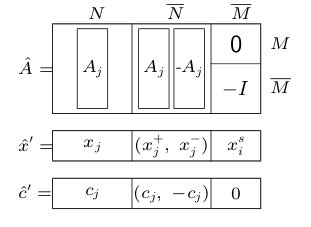
\includegraphics[width=0.6\textwidth]{images/cap5fig53.png}
  \caption{Struttura del problema in forma standard ottenuto da uno in
    forma generale}
  \label{cap5fig53}
\end{figure}

La matrice $\hat{A}$ contiene delle colonne che possiamo classificare
in tre aree:

\begin{itemize}
\item {\bf N}: qui troviamo i coefficienti dei vincoli che avevamo in
  partenza per le variabili $\geq 0$;

\item {\bf $\bar{N}$}: queste colonne sono relative alle variabili
  libere. Tali variabili sono state sostituite da $x_j^+-x_j^-$ e
  dunque si spiega al suo interno la presenza di coefficienti con
  segno positivo $A_j$ e con segno negativo $-A_j$.

\item {\bf $\bar{M}$}: questa colonna conterr\`a degli 0 in
  corrispondenza delle righe che appartenevano a {\em M}, mentre per
  le righe che appartenevano a $\bar{M}$ vi sar\`a $-I$. Ci\`o \`e
  legato all'aggiunta di variabili di surplus che chiaramente hanno
  coefficiente $-1$.
\end{itemize}

Passiamo ad analizzare il vettore $\hat{x}'$. Questo al suo interno
contiene le variabili $x_j$ (quelle per $j \in N$, cio\`e quelle
vincolate ad essere $\geq 0$), poi abbiamo le variabili $x_j^+$ e
$x_j^-$ che sono state aggiunte per sostituire le variabili libere ed
infine abbiamo le variabili di surplus $x_i^-$.

Il vettore $\hat{c}'$ \`e composto dai costi $c_j$ con $j \in N$, dai
coefficienti $c_j$ (al solito per variabili vincolate), $c_j$ e $-c_j$
per variabili libere, 0 per le variabili di surplus.

Vediamo ora di applicare quanto detto in precedenza. Se esiste una
soluzione ottima $\hat{x}^0$ esiste una base $\hat{\mathcal{B}} = \{
\hat{A}_{\hat{\beta}(1)},\dots,\hat{A}_{\hat{\beta}(m)}$ a cui
  corrisponde una sottomatrice $\hat{B} = [\hat{A}_{\hat{\beta}(i)}]$
  tale che $\hat{c}' - \hat{z}' = \hat{c}' - (\hat{c}'_\beta
  \hat{B}^{-1})\hat{A} \geq 0$.

Definendo $\pi' = \hat{c}_\beta'\hat{B}^{-1}$, il vettore $\pi$ deve
essere soluzione ammissibile del problema $\pi'\hat{A} \leq \hat{c}'$
la cui struttura \`e osservabile in figura \ref{cap5fig54}.

\begin{figure}[h!]
  \centering
  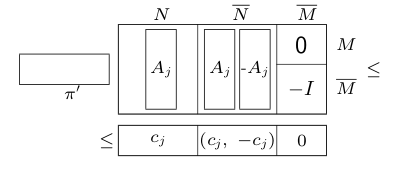
\includegraphics[width=0.7\textwidth]{images/cap5fig54.png}
  \caption{Struttura del problema duale}
  \label{cap5fig54}
\end{figure}

Da questa figura emergono dunque i seguenti vincoli:

\begin{itemize}
  
\item $\pi'A_j \leq c_j$ per $j \in N$
\item coppie $\pi'A_j \leq c_j$ e $-\pi'A_j \leq -c_j$ che implicano
  $\pi'A_j = c_j$ per $j \in \bar{N}$;
\item $-\pi_i \leq 0$ equivalenti a $\pi \geq 0$ per $i \in \bar{M}$;
\item nessun vincolo per $i \in M$, quindi $\pi_i \gtreqless 0$, per
  $i \in M$.

\end{itemize}

Possiamo dunque riassumere le corrispondenze fra problema primale e
problema duale nella seguente tabella:

\vspace{11pt}
\begin{center}
\begin{tabular}{l l l}
{\bf Primale} & & {\bf Duale} \\\hline
$\min c'x$ &  & $\max \pi'b$ \\

$\phantom{min}a_i'x = b_i$ & $i \in M$ & $\phantom{max}\pi_i
\gtreqless 0$ \\

$\phantom{min}a_i'x \geq b_i$ & $i \in \bar{M}$ & $\phantom{max}\pi_i
\geq 0$ \\

$\phantom{min}x_j \geq 0$ & $j \in N$ & $\phantom{max}\pi'A_j \leq
c_j$ \\

$\phantom{min}x_j \gtreqless 0$ & $j \in \bar{N}$ & $\phantom{max}\pi'A_j = c_j$ \\
\end{tabular}
\end{center}
\vspace{11pt}

Notiamo inoltre che:

\begin{itemize}
\item ai costi corrispondono i termini noti e viceversa;
\item i vincoli sono dati dalle righe di {\em A} per il primale, dalle
  colonne di {\em A} per il duale;
\item ad un vincolo corrisponde una condizione su una variabile e
  viceversa;
\item ad una condizione {\em forte} (cio\`e uguaglianza) corrisponde
  una condizione {\em debole} (cio\`e variabile libera) e viceversa.
\end{itemize}

\vspace{11pt}
$\blacktriangleright$ {\bf Esempio}: sia dato il problema primale:

\vspace{11pt}
\begin{center}
\begin{tabular}{l}
$\min z = 2x_1 + x_2 + x_3$\\
$\phantom{min z}x_1 + x_3 = 4$\\
$\phantom{min z}x_2 + 2x_3 \geq 2$\\
$\phantom{min z}x_1,x_2 \geq 0$\\
$\phantom{min z}x_3 \gtreqless 0$\\
\end{tabular}
\end{center}
\vspace{11pt}

Portandolo in forma standard ed applicando l'algoritmo del simplesso
avremo il risultato in figura \ref{cap5tab2}.

\begin{figure}[h!]
  \centering
  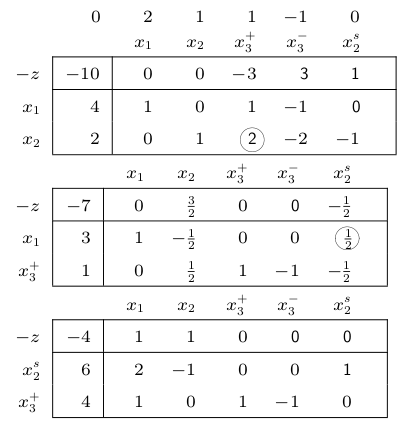
\includegraphics[width=0.7\textwidth]{images/cap5tab2.png}
  \caption{Risoluzione del problema}
  \label{cap5tab2}
\end{figure}

da cui ricaviamo che la soluzione ottima \`e $x_1 = x_2 = 0$, $x_3 =
4$ ed ha valore $z = 4$. 

Costruendo il problema duale otteniamo:

\vspace{11pt}
\begin{center}
\begin{tabular}{l}
$\max w = 4\pi_1 + 2\pi_2$\\
$\phantom{min z}\pi_1 \leq 2$\\
$\phantom{min z}\pi_2 \leq 1$\\
$\phantom{min z}\pi_1 + 2\pi_2 = 1$\\
$\phantom{min z}\pi_1 \gtreqless 0$\\
$\phantom{min z}\pi_2 \geq 0$\\
\end{tabular}
\end{center}
\vspace{11pt}

Si pu\`o eliminare il primo vincolo in quanto implicato dal terzo e
dalla condizione $\pi_2 \geq 0$ e pertanto ridondante. Si procede a
porre il problema in forma standard:

\vspace{11pt}
\begin{center}
\begin{tabular}{l}
$-\min (-w) = -4\pi_1^+ + 4\pi_1^- + 2\pi_2$\\
$\phantom{min z}\pi_2 + \pi_1^s =1$\\
$\phantom{min z}\pi_1^+ - \pi_1^- + 2\pi_2 = 1$\\
$\phantom{min z}\pi_1^+, \pi_1^-, \pi_2, \pi_1^s \geq 0$\\
\end{tabular}
\end{center}
\vspace{11pt}

Si risolve con il simplesso e si ottiene la soluzione $\pi_1 = 1$,
$\pi_2 = 0$ che ha valore $w = 4$. 

Il problema primale ed il duale hanno soluzioni con lo stesso
valore. Non \`e affatto una coincidenza. $\blacktriangleleft$
\vspace{11pt}

\section{Propriet\`a della dualit\`a}

{\bf Teorema:} se un problema di programmazione lineare primale ha
soluzione ottima finita, allora:

\begin{enumerate}
\item anche il suo duale ha soluzione ottima finita;
\item i valori delle due soluzioni sono uguali.
\end{enumerate}

\vspace{11pt}
$\square$ {\bf Dimostrazione}: cosideriamo un problema in forma
standard. Siano $x$ e $\pi$ due soluzioni ammissibili qualunque del
primale e del duale rispettivamente. Dai vincoli duali, $c' \geq
\pi'A$ e da quelli primali $Ax=b$ abbiamo:

\begin{center}
$c'x \geq \pi'Ax = \pi'b$  
\end{center}

Questa relazione esprime la cosiddetta {\bf dualit\`a debole}: il
costo di ogni soluzione ammissibile del primale \`e maggiore o uguale
al costo di ogni soluzione ammissibile del duale. Con una forzatura
potremmo adottare una rappresentazione geometrica nella quale inserire
sia il primale sia il duale. In questa rappresentazione potremmo
osservare chele soluzioni ammissibili e non ottime del primale sono
inammissibili per il duale, mentre quelle ammissibili ma non ottime
del duale sono inammissibili per il primale. Riprendendo l'ultima
formula citata, vediamo che il duale non pu\`o avere soluzione
illimitata. N\`e \`e impossibile poich\'e possiede la soluzione
ammissibile $\pi' = c_\beta'B^{-1}$ (dove {\em B} corrisponde alla
base ottima del primale). Da ci\`o consegue la tesi 1.

\begin{figure}[h!]
  \centering
  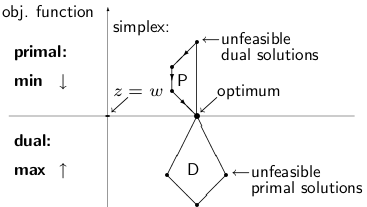
\includegraphics[width=0.66\textwidth]{images/cap5fig55.png}
  \caption{Il mondo primale ed il mondo duale}
  \label{cap5fig55}
\end{figure}

Per quanto riguarda la tesi 2 basta osservare che la soluzione $\pi' =
c_\beta'B^{-1}$ ha costo $\pi'b = c_\beta'B^{-1}b = c_\beta'x_\beta$
uguale al costo ottimo del primale. Come vediamo dalla figura
\ref{cap5fig55} la soluzione ottima \`e l'unica ammissibile per
entrambi i problemi. $\blacksquare$
\vspace{11pt}

{\bf Propriet\`a:} il duale del duale \`e il primale.

\vspace{11pt} $\square${\bf Dimostrazione}: riscriviamo il problema
duale in forma primale:

\vspace{11pt}
\begin{center}
\begin{tabular}{l}
$\min (-b')\pi$\\
$(-A_j')\pi \geq -c_j, j \in N$\\
$(-A_j')\pi = -c_j, j \in \bar{N}$\\
$\pi_i \geq 0, i \in \bar{M}$\\
$\pi_i \gtreqless 0, i \in M$\\
\end{tabular}
\end{center}
\vspace{11pt}

Ora del primale ottenuto scriviamo il duale:

\vspace{11pt}
\begin{center}
\begin{tabular}{l}
$\max x'(-c)\pi$\\
$x_j \geq 0, j \in N$\\
$x_j \gtreqless 0, j \in \bar{N}$\\
$(-a_i')x \leq -b_i, i \in \bar{M}$\\
$(-a_i')x = -b_i, i \in M$\\
\end{tabular}
\end{center}
\vspace{11pt}

Abbiamo riottenuto il duale di partenza. $\blacksquare$
\vspace{11pt}

Adesso possiamo stabilire delle categorie in cui classificare le varie
coppie primale-duale:

\vspace{11pt}
\begin{center}
\begin{tabular}{|l|c|c|c|}
duale/primale & ottimo finito & illimitato & inammissibile \\ \hline
ottimo finito & 1 & NO & NO \\ \hline
illimitato & NO & NO & 3 \\ \hline
inammissibile & NO & 3 & 2 \\ \hline
\end{tabular}
\end{center}
\vspace{11pt}

La prima riga e la prima colonna della tabella derivano da uno dei
teoremi che abbiamo espresso poco fa.  Se il problema primale \`e
illimitato, il problema duale per forza dovr\`a esserlo.  Vediamo
subito come siano possibili anche i casi {\em 1} e {\em
  2}:\vspace{11pt} $\square${\bf Dimostrazione}: riscriviamo il
problema duale in forma primale:

\vspace{11pt}
\begin{center}
\begin{tabular}{l}
$\min (-b')\pi$\\
$(-A_j')\pi \geq -c_j, j \in N$\\
$(-A_j')\pi = -c_j, j \in \bar{N}$\\
$\pi_i \geq 0, i \in \bar{M}$\\
$\pi_i \gtreqless 0, i \in M$\\
\end{tabular}
\end{center}
\vspace{11pt}

Ora del primale ottenuto scriviamo il duale:

\vspace{11pt}
\begin{center}
\begin{tabular}{l}
$\max x'(-c)\pi$\\
$x_j \geq 0, j \in N$\\
$x_j \gtreqless 0, j \in \bar{N}$\\
$(-a_i')x \leq -b_i, i \in \bar{M}$\\
$(-a_i')x = -b_i, i \in M$\\
\end{tabular}
\end{center}
\vspace{11pt}

Abbiamo riottenuto il duale di partenza. $\blacksquare$
\vspace{11pt}

Adesso possiamo stabilire delle categorie in cui classificare le varie
coppie primale-duale:

\vspace{11pt}
\begin{center}
\begin{tabular}{|l|c|c|c|}
\hline
duale/primale & ottimo finito & illimitato & inammissibile \\ \hline
ottimo finito & 1 & NO & NO \\ \hline
illimitato & NO & NO & 3 \\ \hline
inammissibile & NO & 3 & 2 \\ \hline
\end{tabular}
\end{center}
\vspace{11pt}

La prima riga e la prima colonna della tabella derivano da uno dei
teoremi che abbiamo espresso poco fa.  Se il problema primale \`e
illimitato, il problema duale per forza dovr\`a esserlo.  Vediamo
subito come siano possibili anche i casi {\em 2} e {\em 3}:

La coppia:

\vspace{11pt}
\begin{center}
\begin{tabular}{lcl}
$\min x_1$ & $\phantom{aaaaaa}$ & $\max \pi_1 + \pi_2$\\
$\phantom{mina}x_1 + x_2 \geq 1$ && $\phantom{mina}\pi_1 - \pi_2 = 1$ \\
$\phantom{mina}-x_1 - x_2 \geq 1$ && $\phantom{mina}\pi_1 - \pi_2 = 0$\\  
$\phantom{mina}x_1, x_2 \gtreqless 0$ && $\phantom{mina}\pi_1, \pi_2 \geq 0$\\  
\end{tabular}
\end{center}
\vspace{11pt}

in cui sia il primale che il duale contengono vincoli contraddittori,
dimostra come il caso 2 possa verificarsi. Un esempio del caso 3 \`e
mostrato invece dalla coppia:

\vspace{11pt}
\begin{center}
\begin{tabular}{lcl}
$\min x_1$ & $\phantom{aaaaaa}$ & $\max \pi_1 + \pi_2$\\
$\phantom{mina}x_1 + x_2 \geq 1$ && $\phantom{mina}\pi_1 - \pi_2 \leq 1$ \\
$\phantom{mina}-x_1 - x_2 \geq 1$ && $\phantom{mina}\pi_1 - \pi_2 \leq 0$\\  
$\phantom{mina}x_1, x_2 \geq 0$ && $\phantom{mina}\pi_1, \pi_2 \geq 0$\\  
\end{tabular}
\end{center}
\vspace{11pt}

in cui il primale \`e impossibile e il duale \`e illimitato.

\vspace{11pt}
$\blacktriangleright$ {\bf Esempio}: riprendiamo il problema della
dieta:

\vspace{11pt}
\begin{center}
\begin{tabular}{l}
$min\phantom{a}c'x$ \\
$\phantom{mina}Ax= b$ \\
$\phantom{mina}x\geq 0$ \\
\end{tabular}
\end{center}
\vspace{11pt}

in cui il costo $c_j$ \`e il costo di una unit\`a del j-esimo
alimento, $r_i$ il fabbisogno della i-esima sostanza nutritiva ed
$a_{ij}$ la quantit\`a dell'i-esima sostanza contenuta in una unit\`a
del j-esimo alimento. 

Il duale \`e il problema:

\vspace{11pt}
\begin{center}
\begin{tabular}{l}
$\max \pi'r$ \\
$\phantom{mina}\pi'A \leq c'$ \\
$\phantom{mina}\pi \geq 0$ \\
\end{tabular}
\end{center}
\vspace{11pt}

Una possibile interpretazione del duale \`e la seguente: un produttore
di sostanze alimentari vuole metter in commercio m pillole contenenti
ciascuna una delle sostanze nutritive. L'incognita del problema duale
\`e: $\pi_i$, prezzo di vendita per ogni unit\`a dell'i-esima
sostanza, per cui $\pi'r$ \`e il ricavo (da massimizzare) di una
dieta. I vincoli impongono che per ogni alimento {\em j} il costo in
forma di pillole di tutte le sostanze in esso presenti non superi il
costo dell'alimento stesso. $\blacktriangleleft$
\vspace{11pt}

\subsection{Lemma di Farkas}

Piccola parentesi. Nel 1902, cio\`e pi\`u di mezzo secolo prima della
teoria della dualit\`a, il matematico Gyula Farkas dimostr\`o la
seguente propriet\`a:

\begin{quote}
Solo uno dei seguenti sistemi \`e possibile:

\begin{center}
\begin{tabular}{ll}
$(I)\begin{sistema}
Ax=b\\
x \geq 0
\end{sistema}$ &
$(II)\begin{sistema}
y'A \leq 0 \\
b'y > 0
\end{sistema}$
\end{tabular}
\end{center}
\end{quote}

\vspace{11pt} $\square$ {\bf Dimostrazione}: dimostriamo che il
sistema I \`e impossibile se e solo se \`e possibile il sistema
II. Consideriamo la coppia primale duale:

\begin{center}
\begin{tabular}{lp{3cm}l}
{\bf Primale} && {\bf Duale} \\\hline
$\min 0'x$ && $\max b'y$\\
$\phantom{aaa}Ax = b$ && $\phantom{aaa}y'A\leq 0$\\
$\phantom{aaa}x \geq 0$ && $\phantom{aaa}y \gtreqless 0$\\
\end{tabular}
\end{center}

D non \`e impossibile perch\'e la soluzione $y=0$ soddisfa i vincoli
(ma non soddisfa II). Di conseguenza P \`e impossibile se e solo se D
\`e illimitato, ossia il sistema I \`e impossibile se e solo se D \`e
illimitato. Il problmea P, data la sua funzione obiettivo, non pu\`o
avere soluzione strettamente positiva. Di conseguenza se D ha una
soluzione con $b'y > 0$, questa soluzione non pu\`o essere finita (se
lo fosse, per un teorema visto in precedenza, P dovrebbe avere una
soluzione dello stesso valore). Quindi se il sistema II \`e possibile
deve aversi $b'y \rightarrow +\infty$, ossia D \`e illimitato (e il
sistema I \`e impossibile) se e solo se il sistema II \`e
possibile. $\blacksquare$
\vspace{11pt}

Tale dimostrazione fa uso del teorema e della tabella visti nella
sezione precedente pur essendo all'epoca ignoti (la dimostrazione
originale era diversa e un po' pi\`u complessa).


\section{Scarti complementari}

{\bf Teorema degli scarti complementari:} siano $x$ e $\pi$ due
soluzioni ammissibili, rispettivamente del primale e del duale in
forma qualunque. Tali soluzioni sono entrambe ottime {\bf se e
  soltanto se}:

\begin{equation}
  \label{c1}
  u_i = \pi_i(a_i'x-b_i) = 0, \phantom{aaa}i=1,\dots,m
\end{equation}

\begin{equation}
  \label{c2}
  v_j = (c_j-\pi'A_j) = 0, \phantom{aaa}j=1,\dots,1
\end{equation}

\vspace{11pt} $\square$ {\bf Dimostrazione}: si osservi che $u_i \geq
0 \forall i$. Allo stesso modo si vede facilmente che $v_i \geq 0
\forall j$. Valgono quindi le relazioni:

\begin{center}
$U = \sum\limits_{i=1}^m u_i \geq 0 \phantom{aaaaaaa}V =
  \sum\limits_{j=1}^n v_j \geq 0$  
\end{center}

da cui si ha che $U = V = 0$ vale se e solo se le due relazioni nella
tesi del teorema valgono. Consegue:


\begin{center}
$U + V = \sum\limits_{i=1}^m \pi_i (\sum\limits_{j=1}^n a_{ij}x_j -
  b_i) + \sum\limits_{j=1}^n (c_j - \sum\limits_{i=1}^m
  \pi_ia_{ij})x_j =$

$\sum\limits_{i=1}^m\sum\limits_{j=1}^n\pi_ia_{ij}x_j -
  \sum\limits{i=1}^m \pi_ib_i + \sum\limits_{j=1}^n c_jx_j -
  \sum\limits_{j=1}^n\sum\limits_{i=1}^m \pi_i a_{ij} x_j = c'x- \pi'b$
\end{center}

cio\`e le relazioni enunciate nella tesi valgono se e solo se $\pi'b =
c'x$, quindi (per il primo teorema introdotto in questo capitolo) se e
solo se $x$ e $\pi$ sono ottime.  $\blacksquare$
\vspace{11pt}

Questo teorema afferma che per ogni {\em i} l'i-esima variabile duale
\`e nulla o l'i-esimo vincolo primale \`e soddisfatto con uguaglianza
e per ogni {\em j} o il j-esimo vincolo duale \`e soddisfatto con
uguaglianza o la j-esima variabile primale \`e nulla. Si supponga ad
esempio di aver trovato la soluzione {\em x} del primale. Per ogni $j$
tale che $x_j > 0$, nella soluzione ottima del duale deve valere
$\pi'A_j = c_j$. Si supponga invece di possedere la soluzione $\pi$
del duale: per ogni $j$ tale che $\pi'A < c_j$, nella soluzione ottima
del primale deve valere $x_j = 0$. Relazioni analoghe valgono fra
vincoli primali e variabili duali. $\blacktriangleleft$
\vspace{11pt}

\vspace{11pt}
$\blacktriangleright$ {\bf Esempio}: consideriamo il seguente
problema:

\vspace{11pt}
\begin{center}
\begin{tabular}{l}
$\min z = 2x_1 + x_2 + x_3$\\
$\phantom{min}x_1 + x_3 = 4$\\
$\phantom{min}x_2 + 2x_3 \geq 2$\\
$\phantom{min}x_1, x_2 \geq 0$\\
$\phantom{min}x_3 \gtreqless 0$\\
\end{tabular}
\end{center}
\vspace{11pt}

Il vincolo $x_1 + x_3 = 4$ garantisce che la prima delle due
condizioni \`e soddisfatta da qualunque $\pi$ e quindi non fornisce
informazioni. La soluzione ottima trovata, $x_1 = x_2 = 0, x_3 = 4$,
garantisce che delle tre condizioni (\ref{c2}), le prime due sono
soddisfatte da qualunque $\pi$ ammissibile. Restano non casualmente
due equazioni in que incognite:

\begin{itemize}
\item la seconda condizione \ref{c2}, $\pi_2(x_2 + 2x_3 - 2) = 0$, da
  cui si ricava $\pi_2 = 0$;
\item la terza condizione \ref{c1}, $(1-(\pi_1 + 2\pi_2))x_3 = 0$, da
  cui si ricava $\pi_1 = 1$ che completa la soluzione ottima del
  duale
\end{itemize}
$\blacktriangleleft$
\vspace{11pt}

\vspace{11pt}
$\blacktriangleright$ {\bf Esempio}: consideriamo il seguente esempio:

\vspace{11pt}
\begin{center}
\begin{tabular}{l}
$\min z = -x_1 - 2x_2$\\
$\phantom{min}x_1 + x_2 + x_3 = 2$\\
$\phantom{min}x_1 + 3x_2 + x_4 = 3$\\
$\phantom{min}3x_2 + x_5 = 2$\\
$\phantom{min}x_1, x_2, x_3, x_4, x_5 \geq 0$\\
\end{tabular}
\end{center}
\vspace{11pt}

per il quale la soluzione ottima \`e $x' =
(\frac{3}{2},\frac{1}{2},0,0,\frac{1}{2})$ di valore $z =
-\frac{5}{2}$. Scriviamone il duale:

\vspace{11pt}
\begin{center}
\begin{tabular}{l}
$\max w = 2\pi_1 + 3\pi_2 + 2\pi_3$\\
$\phantom{min}\pi_1 + \pi_2 \leq -1$\\
$\phantom{min}\pi_1 + 3\pi_2 + 3\pi_3 \leq -2$\\
$\phantom{min}\pi_1 \leq 0$\\
$\phantom{min}\pi_2 \leq 0$\\
$\phantom{min}\pi_3 \leq 0$\\
$\phantom{min}\pi_1, \pi_2, \pi_3 \gtreqless 0$\\
\end{tabular}
\end{center}
\vspace{11pt}

Il primale \`e in forma standard, per cui tutte le \ref{c1} sono
automaticamente soddisfatte. La soluzione trovata garantisce che,
delle cinque condizioni \ref{c2}, la terza e la quart asono
soddisfatte da qualunque $\pi$ ammissibile. Restano tre equazioni
(prima, seconda e quinta della \ref{c2}) in tre incognite:

\begin{itemize}
\item $(-1-\pi_1-\pi_2)\frac{3}{2} = 0$
\item $(-2-\pi_1-3\pi_2-3\pi_3)\frac{1}{2} = 0$
\item $(0-\pi_3)\frac{1}{2} = 0$
\end{itemize}

Risolvendo il sistema risultante si ottiene (considerando che dalla
terza $\pi_3 = 0$) la soluzione $\pi_1 = \pi_2 = -\frac{1}{2}$ di
valore $-\frac{5}{2}$. $\blacktriangleleft$
\vspace{11pt}


\section{Algoritmo del simplesso duale}

L'algoritmo del simplesso duale \`e un algoritmo simmetrico
all'algoritmo del simplesso visto fino a questo momento. Inizia con
una soluzione ammissibile per il duale (che soddisfa dunque il
criterio di ottimalit\`a) e che tramite pivoting porta la soluzione
verso l'ammissibilit\`a per il primale.

Vediamo i passi dell'algoritmo tramite un esempio numerico.

\begin{enumerate}
\item Iniziamo con una base ammissibile per il duale, cio\`e con costi
  relativi maggiori di 0, ma non ammissibile per il primale, ossia con
  almeno una variabile in base con valore minore di 0.

\begin{figure}[h!]
  \centering
  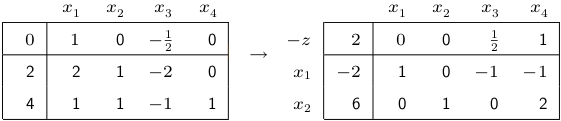
\includegraphics[width=0.7\textwidth]{images/cap5tab3.png}
  \caption{Figura d'esempio}
  \label{cap5tab3}
\end{figure}

\item Dato che vogliamo eliminare le inammissibilit\`a contenute nel
  tableau, scegliamo una riga $i \geq 1$ corrispondente ad un $y_{i0}
  < 0$, nel nostro caso la riga 1 dato che $y_{11} = -2$. 

\item Vogliamo che il pivoting renda positiva $y_{i0}$, per cui
  scegliamo la colonna {\em s} del pivot $y_{is}$ tra le colonne a cui
  corrisponde un valore negativo. Nel nostro caso abbiamo due colonne
  a cui corrisponde il valore -1 ($y_{13}$ e $y_{14}$).

\item Nella riga 0, in corrispondenza della colonna scelta al passo
  precedente dovremo avere 0. Lo porter\`a il pivoting tramite
  la solita operazione:

  \begin{center}
    $\tilde{y}_{0j} := y_{0j} -
    \bigr(\frac{y_{0s}}{y_{is}}\bigr)y_{ij}\phantom{aaaaaaa}(j=1,\dots,n)$
  \end{center}

  Il pivoting deve inoltre mantenere la non-negativit\`a di
  $\tilde{y}_{0j}$ per $j=1,\dots,n$. Imponendo $\tilde{y}_{0j} \geq
  0$ si ha:

  \begin{center}
    $\frac{y_{0j}}{y_{ij}} \leq \frac{y_{0o}}{y_{is}} \forall j :
    y_{ij}<0$
  \end{center}

  In conclusione il pivot viene scelto come:

  \begin{center}
    $\max\limits_{j:y_{ij}<0}\bigr\{\frac{y_{0j}}{y_{ij}}\bigr\} = \frac{y_{0s}}{y_{is}}$
  \end{center}


\item 

\end{enumerate}

Questo \`e dunque l'algoritmo:

\small
\vspace{11pt}
\begin{center}
\begin{tabular}{||l||}
\hline\hline
{\bf procedure DUAL SIMPLEX}:\\
{\bf comment}: we are given a tableau such that $y_{0j} \geq 0 \forall j and \exists i > 0 : y_{i0} < 0$;\\
{\bf begin}\\
\phantom{aa}optimal := false;\\
\phantom{aa}infeasible := false;\\
\phantom{aa}{\bf while} optimal = {\bf false} and infeasible = {\bf false} {\bf do}\\
\phantom{aaaa}{\bf if} $y_{i0} \geq 0$ for i = 1,\dots,m {\bf then} optimal = {\bf true}\\
\phantom{aaaa}{\bf else}\\
\phantom{aaaaaa}{\bf begin}\\
\phantom{aaaaaaaa}{\bf select} an i > 0 : $y_{i0} < 0$;\\
\phantom{aaaaaaaa}{\bf if} $y_{ij} \geq 0$ for j = 1, \dots, n {\bf
  then}\\
\phantom{aaaaaaaaaa} infeasible := {\bf true} ({\bf comment}: unbounded dual)\\
\phantom{aaaaaaaa}{\bf else} $\vartheta := \max\limits_{j>0:y_{ij}<0} \bigr \{
\frac{y_{0j}}{y_{ij}} \} = \frac{y_{0s}}{y_{is}}$, e pivoting su $y_{is}$\\
\phantom{aaaaaa}{\bf end}\\
{\bf end.}\\
\hline\hline
\end{tabular}
\end{center}
\vspace{11pt}
\normalsize

\section{Algoritmo primale-duale}


\subsection{Fase1: Inizializzazione}

Per iniziare tale algoritmo ci occorre soltanto una soluzione $\pi$
ammissibile per D. Se $c_j \geq 0 \forall j$, la soluzione duale nulla
$\pi = 0$ \`e ammissibile. In caso contrario possiamo trasformare P in
un problema equivalente aggiungendo una nuova variabile $x_{n+1}$ con
costo $c_{n+1} = 0$ ed un nuovo vincolo $x_1 + \dots + x_n + x_{n+1} =
b_{m+1}$ dove $b_{m+1} = M$ (valore molto grande, ad esempio un
infinito di macchina).

\vspace{11pt}
\begin{center}
\begin{tabular}{l}
$\min z = c'x + 0$\\
$\phantom{min}Ax = b$\\
$\phantom{min}\sum\limits_{j=1}^n x_j + x_{n+1} = b_{m+1}$\\
$\phantom{min}x \geq 0$\\
$\phantom{min}x_{n+1} \geq 0$\\
\end{tabular}
\end{center}
\vspace{11pt}

Il problema che ricaviamo in questo modo \`e equivalente a quello dato
in quanto:

\begin{itemize}
\item ha la stessa funzione obiettivo;
\item per ogni $\bar{x}$ ammissibile per il problema orginale,
  aggingendo $\bar{x}_{n+1} = b_{m+1} - \sum\limits_{j=1}^n \bar{x}_j$
  si ottiene una nuova soluzione che soddisfa il vincolo.
\end{itemize}

Il duale di questo problema ha soluzione ammissibile $\pi_i = 0$ per
$i=1,\dots,m$ e $\pi_{m+1} = \min_j\{c_j\} (<0)$.


\subsection{Fase2: Primale Ristreto (RP)}

Data una soluzione ammissibile per il duale $\pi$, sia:

\begin{center}
$J = \{ j : \pi'A_j = c_j \}$
\end{center}

Questo insieme \`e costituito da tutte le {\em j} tali per cui il
prodotto della soluzione $\pi'$ per la colonna $j$ della matrice $A$
d\`a come risultato il costo $c_j$.

Una soluzione $x$ ammissibile per il primale P \`e ottima se e solo se
$x_j = 0$ per tutte le $j$ che non fanno parte dell'insieme $J$
individuato. Si vuole trovare quindi una soluzione $x$ che soddisfi:

\begin{center}
$\begin{sistema}
Ax = b\\
x \geq 0\\
x_j = 0 \forall j \not\in J
\end{sistema}$
\end{center}

cio\`e:

\begin{center}
$\begin{sistema}
\sum\limits_{j \in J} a_{ij}x_j = b_i\phantom{aa}(i=1,\dots,m)\\
x_j \geq 0\phantom{aa}(j \in J)
\end{sistema}$
\end{center}

Per trovare questa soluzione si risolve un problema LP detto {\bf
  Primale Ristretto} che ricorda quello della prima fase
dell'algoritmo del simplesso: introduciamo $m$ variabili artificiali
$x_i^a$ (i=1,\dots,m) e definiamo Primale Ristretto il seguente
problema:

\vspace{11pt}
\begin{center}
\begin{tabular}{l}
$\min \zeta = \sum\limits_{i=1}^m x_i^a$\\
$\phantom{min}\sum\limits_{j\in J} a_{ij}x_{j} + x_i^a = b_i$,
  $(i=1,\dots,m)$\\
$\phantom{min}x_j \geq 0$, $j \in J$\\
$\phantom{min}x_i^a \geq 0$, $(i=1,\dots,m)$\\
\end{tabular}
\end{center}
\vspace{11pt}

Se la soluzione ottima \`e $\zeta_{opt} = 0$, $x$ e $\pi$ risolvono P
e D e l'algoritmo termina. Altrimenti significa che non esiste alcun
{\em x} che con il $\pi$ attuale soddisfi \ref{c1} e \ref{c2} quindi
il $\pi$ attuale non \`e quello ottimo. Come al solito un esempio
chiarisce meglio le idee.

\vspace{11pt}$\blacktriangleright$ {\bf Esempio:} Consideriamo la
coppia primale-duale:

\begin{center}
\begin{tabular}{lp{3cm}l}
$(P)\phantom{a}\min z = 2x_1 + x_2 + 3x_3$ && $(D)\phantom{a}\max w =
  4\pi_1+\pi_2$\\
$\phantom{(p)mina}x_1 + 2x_2 = 4$ && $\phantom{(p)mina}\pi_1 + \pi_2 \leq 2$\\
$\phantom{(p)mina}x_1 - x_2 + x_3 = 1$ && $\phantom{(p)mina}2\pi_1 - \pi_2 \leq 1$ \\
$\phantom{(p)mina}x_1,x_2,x_3 \geq 0$ && $\phantom{(p)mina}\pi_2 \leq 3$\\
&& $\phantom{(p)mina}\pi_1, \pi_2 \gtreqless 0$
\end{tabular}
\end{center}

Iniziamo con $\pi_1 = \pi_2 = 1$ (ammissibile per D), da cui $J =
\{1,2\}$ e risolviamo il primale ristretto:

\vspace{11pt}
\begin{center}
\begin{tabular}{l}
$(RP)\phantom{a}\min \zeta = x_1^a + x_2^a$\\
$\phantom{(p)mina}x_1 + 2x_2 + x_1^a = 4$\\
$\phantom{(p)mina}x_1 - x_2 + x_2^a = 1$\\
$\phantom{(p)mina}x_1,x_2,x_1^a,x_2^a \geq 0$\\
\end{tabular}
\end{center}
\vspace{11pt}

La cui risoluzione \`e in figura \ref{cap5tab58}.

\begin{figure}[h!]
  \centering
  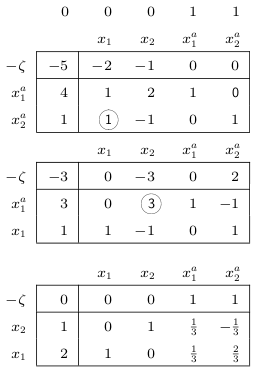
\includegraphics[width=0.6\textwidth]{images/cap5tab58.png}
  \caption{Risoluzione dell'RP}
  \label{cap5tab58}
\end{figure}

La soluzione ottima di valore nullo trovata, $x' = (2,1,0)$, e la
soluzione duale attuale $\pi' = (1,1)$ soddisfano le condizioni
\ref{c1} e \ref{c2} dunque sono ottime. $\blacktriangleleft$
\vspace{11pt}

\vspace{11pt}$\blacktriangleright$ {\bf Esempio:} Consideriamo la
coppia primale-duale:

\begin{center}
\begin{tabular}{lp{3cm}l}
$(P)\phantom{a}\min z = x_1 + x_3$ && $(D)\phantom{a}\max w =
  5\pi_1+6\pi_2$\\
$\phantom{(p)mina}x_1 + 2x_2 + x_4 = 5$ && $\phantom{(p)mina}\pi_1 \leq 1$\\
$\phantom{(p)mina}x_2 + 2x_3 = 6$ && $\phantom{(p)mina}2\pi_1 + \pi_2 \leq 0$ \\
$\phantom{(p)mina}x_1,x_2,x_3,x_4 \geq 0$ && $\phantom{(p)mina}2\pi_2 \leq 1$\\
&& $\phantom{(p)mina}\pi_1 \leq 0$\\
&& $\phantom{(p)mina}\pi_1, \pi_2 \gtreqless 0$
\end{tabular}
\end{center}

Iniziamo con $\pi_1 = \pi_2 = 0$, da cui $J = \{2,4\}$ e risolviamo il
primale ristretto:

\vspace{11pt}
\begin{center}
\begin{tabular}{l}
$(RP)\phantom{a}\min \zeta = x_1^a + x_2^a$\\
$\phantom{(p)mina}2x_2 + x_4 + x_1^a = 5$\\
$\phantom{(p)mina}x_2 + x_2^a = 6$\\
$\phantom{(p)mina}x_2,x_4,x_1^a,x_2^a \geq 0$\\
\end{tabular}
\end{center}
\vspace{11pt}

La cui risoluzione \`e in figura \ref{cap5tab59}.

\begin{figure}[h!]
  \centering
  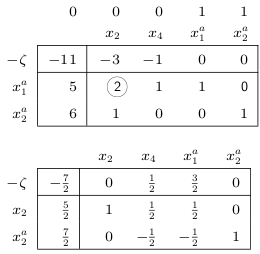
\includegraphics[width=0.6\textwidth]{images/cap5tab59.png}
  \caption{Risoluzione dell'RP}
  \label{cap5tab59}
\end{figure}

La soluzione ottima non vale 0, pertanto la soluzione $\pi$ attuale
non \`e quella ottima. Osserviamo che la riga 0 iniziale e il tableau
finale forniscono la soluzione ottima del duale del primale
ristretto. $\blacktriangleleft$
\vspace{11pt}

\subsection{Fase3: Duale del Primale Ristretto (DRP)}

Se la soluzione ottima del primale ristretto \`e maggiore di zero
occorre correggere la soluzione attuale del duale. Consideriamo dunque
il duale del problema ristretto:

\vspace{11pt}
\begin{center}
\begin{tabular}{l}
$\max \pi'b$\\
$\phantom{min}\pi'A_j \leq 0, (j\in J)$\\
$\phantom{min}\pi_i \leq 1, (i=1,\dots,m)$\\
$\phantom{min}\pi_i \gtreqless 0, (i=1,\dots,m)$\\
\end{tabular}
\end{center}
\vspace{11pt}

Sia $\bar{\pi}$ la soluzione ottima del duale del problema ristretto
(che chiamiamo DRP) fornita dalla soluzione del RP. Il nostro intento
\`e quello di ritentare con una nuova soluzione $\pi^*$ data da:

\begin{center}
$\pi^* = \pi + \vartheta\bar{\pi}$
\end{center}

determinando $\vartheta$ in modo che $\pi^*$ resti ammissibile per il
duale e che il costo del duale aumenti.

Il secondo punto \`e facile da affrontare: il costo della nuova
soluzione sar\`a:

\begin{center}
$\pi^* \phantom{.}' b = \pi'b + \vartheta\bar{\pi}'b$
\end{center}

dove $\bar{\pi}'b = \zeta_{opt}$ (RP e DRP hanno lo stesso valore
ottimo). Dovremo dunque avere $\vartheta > 0$.

Per quanto riguarda invece il primo punto, cio\`e far in modo che la
soluzione resti ammissibile per il problema duale, occorre che valga
$\pi^* \phantom{.}' A_j \leq c_j$ per $j=1,\dots,n$, cio\`e:

\begin{center}
$\pi'A_j + \vartheta \bar{\pi}'A_j \leq c_j$, (j=1,\dots,n)
\end{center}

Possiamo dunque fare due osservazioni:

\begin{itemize}

\item se $\bar{\pi}'A_j \leq 0, \forall j$, $\vartheta$ pu\`o crescere
  illimitatamente mantenendo l'ammissibilit\`a e quindi il nuovo costo
  di D pu\`o tendere all'infinito. In tal caso possiamo dunque
  concludere che il primale \`e impossibile. D'altra parte sappiamo
  che $\bar{\pi}$ \`e soluzione ammissibile (e ottima) del DRP, per
  cui sicuramente soddisfa $\bar{\pi}'A_j \leq 0$ per tutti i $j \in
  J$. In conclusione:

  \begin{quote}
    Se $\zeta_{opt} > 0$ in RP e la soluzione ottima $\bar{\pi}'$ del
    suo duale DRP soddisfa $\bar{\pi}'A_j \leq 0 \forall j \not\in J$,
    allora P \`e impossibile.
  \end{quote}

\item se invece esistono degli indici $j \not\in J$ per i quali si ha
  $\bar{\pi}' A_j > 0$, occorre che per tutti questi $j$ -i abbia
  $\pi'A_j + \vartheta\bar{\pi}'A_j \leq c_j$, cio\`e $\vartheta \leq
  (c_j - \pi'A_j)/\bar{\pi}'A_j$. Pertanto:

  \begin{quote}
    Se $\zeta_{opt} > 0$ in RP ed $\exists j \not \in J :
    \bar{\pi}'A_j > 0$, allora il massimo $\vartheta$ che mantiene
    l'ammissibilit\`a \`e:

    \begin{center}
      \begin{equation}
      \vartheta^* = \min\limits_{j\not\in J : \bar{\pi}'A_j > 0}
      \bigr\{ \frac{c_j - \pi'A_j}{\bar{\pi}'A_j} \bigr\}
      \ref{alg}
      \end{equation}
    \end{center}

    e il costo della nuova soluzione \`e $w^* = w +
    \vartheta^*\bar{\pi}'b > w$.
  \end{quote}

\end{itemize}

\subsection{Algoritmo}

\small
\begin{center}
\begin{tabular}{||l||}
\hline\hline
{\bf procedure Primale Duale:}\\
{\bf begin}\\
\phantom{aa}{\bf comment:} inizializzazione\\
\phantom{aa}{\bf for each} $b_i < 0$ {\bf do} moltiplica l'i-esima equazione per -1;\\
\phantom{aa}determina una soluzione $\pi$ ammissibile per il duale;\\
\phantom{aa}ottimo := impossibile := {\em false};\\
\phantom{aa}{\bf while} ottimo = {\em false} {\bf and} impossible = {\em false} {\bf do}\\
\phantom{aaaa}{\bf begin}\\
\phantom{aaaaaa}{\bf comment:} Primale ristretto\\
\phantom{aaaaaa}$J := \{j : \pi'A_j = c_j \};$\\
\phantom{aaaaaa}{\bf call Simplesso} per il problema RP e sia $\bar{\pi}$ la soluzione di DRP;\\
\phantom{aaaaaa}{\bf if} $\zeta_{opt} = 0$ {\bf then} ottimo = {\em true}\\
\phantom{aaaaaa}{\bf else} ({\bf comment:} Duale del primale ristretto)\\
\phantom{aaaaaaaa}{\bf if} $\bar{\pi}'A_j \leq 0 \forall j \not\in J$ {\bf then} impossible := {\em true}\\
\phantom{aaaaaaaa}{\bf else} $\vartheta = \min\limits_{j\not\in J : \bar{\pi}'A_j > 0} \bigr\{\frac{c_j - \pi'A_j}{\bar{\pi}'A_j} \bigr\}; \pi := \pi + \vartheta \bar{\pi}$\\
\phantom{aaaa}{\bf end}\\
{\bf end.}\\
\hline\hline
\end{tabular}
\end{center}
\normalsize

\vspace{11pt}$\blacktriangleright$ {\bf Esempio:} riprendiamo l'ultimo
esempio visto. Il duale \`e:

\vspace{11pt}
\begin{center}
\begin{tabular}{l}
$\max 5\pi_1 + 6\pi_2$\\
$2\pi_1 + \pi_2 \leq 0$\\
$\pi_1 \leq 0$\\
$\pi_1 \leq 1$\\
$\pi_2 \leq 1$\\
$\pi_1,\pi_2 \gtreqless 0$\\
\end{tabular}
\end{center}
\vspace{11pt}

La soluzione del duale \`e $\bar{\pi_1} = -\frac{1}{2}, \bar{\pi_2} =
1$. Ritentiamo con una soluzione duale data da $\pi_1^* = 0 +
\vartheta\cdot (-\frac{1}{2}), \pi_2^* = 0 + \vartheta\cdot 1$, con
$\vartheta > 0$ e tale che $\pi^*$ soddisfi i quattro vincoli di D
(ancora una volta rifarsi all'esempio precedente).

Poich\'e $J = \{ 2, 4\}$, il secondo e quarto vincolo sono certamente
soddisfatti. Per il primo risulta $\bar{\pi}'A_1<0$. La formula
\ref{alg} considera solo il terzo vincolo e si ottiene $\vartheta^* =
\frac{1}{2}$, da cui $\pi_1^*= - \frac{1}{4}, \pi_2^* =
-\frac{1}{2}$. Il nuovo costo di D \`e $\frac{7}{4}$ (dato da $0 +
\frac{1}{2} \cdot \frac{7}{2}$). Otteniamo $J = \{ 2,3\}$ e il nuovo
primale ristretto:

\vspace{11pt}
\begin{center}
\begin{tabular}{l}
$(RP)\phantom{a}\min z = x_1^a + x_2^a$\\
$\phantom{RPamin}2x_2 + x_1^a = 5$\\
$\phantom{RPamin}x_2 + 2x_3 + x_2^a = 6$\\
$\phantom{RPamin}x_2, x_3, x_1^a, x_2^a \geq 0$\\
\end{tabular}
\end{center}
\vspace{11pt}

\begin{figure}[h!]
  \centering
  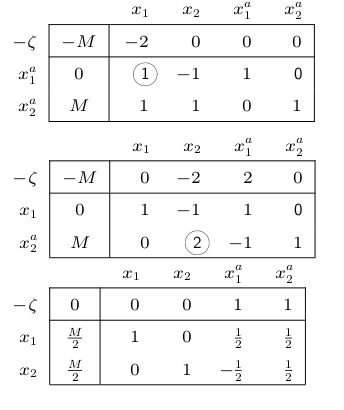
\includegraphics[width=0.6\textwidth]{images/cap5tab87.png}
  \caption{Risoluzione dell'RP}
  \label{cap5tab87}
\end{figure}

La risoluzione di tale problema \`e mostrata in figura
\ref{cap5tab87}. La soluzione ottima \`e $x' =
(0,\frac{5}{2},\frac{7}{4},0)$, quella di D \`e $\pi' =
(-\frac{1}{4},\frac{1}{2})$. Il valore delle due soluzioni \`e
$\frac{7}{4}$. $\blacktriangleleft$\vspace{11pt}

\subsection{Considerazioni}

Facciamo alcune considerazioni sull'algoritmo e sull'esempio appena
visto. L'algoritmo pu\`o terminare con:

\begin{itemize}
\item ottimo finito per primale e duale;
\item duale illimitato, dunque primale impossibile.
\end{itemize}

Non sono quindi previste due delle situazioni viste nella tabella in
sezione 5.3, cio\`e il caso in cui il primale ed il duale siano
impossibili ed il caso in cui il primale sia illimitato ed il duale
impossibile. Entrambe le situazioni non considerate si riferiscono a
casi in cui il duale \`e impossibile, mentre noi abbiamo costruito
nella fase di inizializzazione la soluzione duale
ammissibile. Costruendo noi una soluzione duale ammissibile stiamo
falsando il problema evitando i due casi di duale impossibile? La
risposta \`e nel valore {\em M} (idealmente infinito) introdotto per
contruire la soluzione ideale e nell'aggiunta di una variabile ed un
vincolo addizionali. Tali operazioni rendono {\em apparentemente}
possibile costruire una soluzione duale ammissibile anche in casi in
cui il duale \`e effettivamente impossibile, ma:

\begin{itemize}
\item nel caso in cui il primale ed il duale siano entrambi
  impossibili l'algoritmo termina con ``impossibile = {\em true}'';

\item nel caso in cui il duale sia impossibile ed il primale
illimitato, l'algoritmo termina con ``ottimo = {\em true}'', ma il
tableau contiene variabili con valore infinito per cui il primale \`e
illimitato.
\end{itemize}

L'algoritmo fornisce dunque sempre la soluzione corretta del problema
primale.

\vspace{11pt}$\blacktriangleright$ {\bf Esempio:} consideriamo il
problema primale illimitato:

\vspace{11pt}
\begin{center}
\begin{tabular}{l}
$min\phantom{a}-x_1-x_2$ \\
$\phantom{mina}x_1-x_2 \leq 0 \rightarrow x_1 - x_2 + x_3 = 0$ \\
$\phantom{mina}x_1,x_2 \geq 0 \rightarrow x_1,x_2,x_3 \geq 0$ \\
\end{tabular}
\end{center}
\vspace{11pt}

L'inizializzazione produce i problemi primale e duale:

\vspace{11pt}
\begin{tabular}{lp{3cm}l}
$\min -x_1-x_2$ & & $\max M\pi_2$ \\
$\phantom{mina}x_1-x_2+x_3 = 0$ && $\phantom{mina}\pi_1+\pi_2 \leq -1$
  \\
$x_1 + x_2 + x_3 + x_4 = M$ && $-\pi_1 + \pi_2 \leq -1$ \\
$x_1, x_2, x_3, x_4 \geq 0$ && $\pi_1 + \pi_2 \leq 0$ \\
& & $\pi_2\leq0$\\
& & $\pi_1,\pi_2 \gtreqless 0$
\end{tabular}
\vspace{11pt}

e la soluzione duale $\pi_1 = 0, \pi_2 = \min\{ c_j \} = -1$, da cui
$J = \{1,2\}$:

\vspace{11pt}
\begin{center}
\begin{tabular}{l}
$(RP)\phantom{aa}\min x_1^a + x_2^a$ \\
$\phantom{(RP)aamina}x_1 - x_2 + x_1^a = 0$ \\
$\phantom{(RP)aamina}x_1 + x_2 + x_2^a = M$ \\
$\phantom{(RP)aamina}x_1, x_2, x_1^a, x_2^a \geq 0$ \\
\end{tabular}
\end{center}
\vspace{11pt}

La risoluzione del Primale Ristretto \`e mostrata in figura
\ref{cap5tab511}.

\begin{figure}[h!]
  \centering
  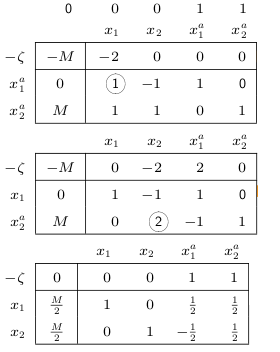
\includegraphics[width=0.6\textwidth]{images/cap5tab511.png}
  \caption{Risoluzione dell'RP}
  \label{cap5tab511}
\end{figure}

La soluzione primale ottima trovata dall'algoritmo \`e dunque $x_1 =
x_2 = \frac{M}{2} (\rightarrow -\infty)$ di valore $z = -M
(\rightarrow -\infty)$. $\blacktriangleleft$\vspace{11pt}


\vspace{11pt}$\blacktriangleright$ {\bf Esempio:} consideriamo ora una
situazione in cui si il primale che il duale siano impossibili. 

\vspace{11pt}
\begin{center}
\begin{tabular}{l}
$min\phantom{a}x_1 - 2x_2$ \\
$\phantom{mina}x_1-x_2 \geq 1 \rightarrow x_1 - x_2 - x_3 = 1$ \\
$\phantom{mina}-x_1 + x_2 \geq 1 \rightarrow -x_1 + x_2 - x_4 = 1$ \\
$\phantom{mina}x_1,x_2 \geq 0 \rightarrow x_1,x_2,x_3,x_4 \geq 0$ \\
\end{tabular}
\end{center}
\vspace{11pt}

Si vede facilmente che anche il problema duale \`e impossibile in
quanto contiene i vincoli:

\begin{center}
$\pi_1 - \pi_2 \leq 1$ \\
$-\pi_1 + \pi_2 \leq -2$
\end{center}

L'inizializzazione del problema primale produce:

\vspace{11pt}
\begin{center}
\begin{tabular}{l}
$(P)\phantom{a}\min x_1-2x_2$ \\
$\phantom{(P)amina}x_1-x_2-x_3 = 1$\\
$\phantom{(P)amina}-x_1+x_2-x_4 = 1$\\
$\phantom{(P)amina}x_1 + x_2 + x_3  + x_4 + x_5 = M$\\
$\phantom{(P)amina}x_1, x_2, x_3, x_4, x_5 \geq 0$
\end{tabular}
\end{center}
\vspace{11pt}

e il suo duale:

\vspace{11pt}
\begin{center}
\begin{tabular}{l}
$(P)\phantom{a}\max \pi_1 + \pi_2 + M\pi_3$ \\
$\phantom{(P)amina}\pi_1 - \pi_2 + \pi_3 \leq 1$\\
$\phantom{(P)amina}-\pi_1 + \pi_2 + \pi_3 \leq -2$\\
$\phantom{(P)amina}-\pi_1 + \pi_3 \leq 0$\\
$\phantom{(P)amina}-\pi_2 + \pi_3 \leq 0$\\
$\phantom{(P)amina}\pi_3 \leq 0$\\
$\phantom{(P)amina}\pi_1,\pi_2,\pi_3 \gtreqless 0$
\end{tabular}
\end{center}
\vspace{11pt}

La soluzione duale ammissibile iniziale \`e quindi $\pi_1 = \pi_2 = 0,
\pi_3 = \min \{ c_j\} = -2$ da cui $J = \{ 2\}$. La risoluzione del
primale ristretto \`e in figura \ref{cap5tab512}.

\begin{figure}[h!]
  \centering
  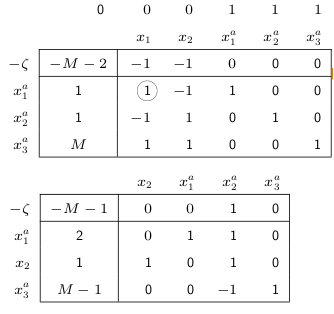
\includegraphics[width=0.6\textwidth]{images/cap5tab512.png}
  \caption{Risoluzione dell'RP}
  \label{cap5tab512}
\end{figure}

La soluzione ottimale non vale 0 per cui bisogna modificare la
soluzione duale attuale. La soluzione duale del primale ristretto \`e
$\bar{\pi}' = (1,0,1)$, da cui si ottiene $\vartheta = \min
\{\frac{3}{2}, \frac{1}{2} \} = \frac{3}{2}$. La nuova soluzione duale
\`e pertanto $\pi' = (\frac{3}{2},0,-\frac{1}{2})$. Si ottiene $J = \{
1,2\}$. Risolviamo il nuovo primale ristretto come mostrato in figura
\ref{cap5tab512bis}.

\begin{figure}[h!]
  \centering
  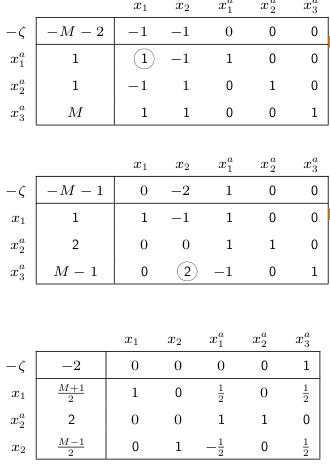
\includegraphics[width=0.6\textwidth]{images/cap5tab512bis.png}
  \caption{Risoluzione dell'RP}
  \label{cap5tab512bis}
\end{figure}

Anche in questo caso la soluzione ottima non vale 0. La soluzione del
duale del primale ristretto \`e $\bar{\pi}' = (1,1,0)$. In questo caso
si verifica che $\bar{\pi}'A_j \leq 0 \forall j$. Di conseguenza il
primale \`e impossibile. $\blacktriangleleft$\vspace{11pt}

\end{document}
